% Klaro - Major Project Report (JIIT, Dept. of CSE & IT)
% Format follows "Final major & instructions_Odd2025": A4, 11 pt text, 13 pt bold main headings,
% 12 pt bold sub-headings, 1.5 line spacing, margins L 3.5 cm / T 2.5 cm / R 1.25 cm / B 1.25 cm,
% roman numbers from the Abstract, first page of each chapter unnumbered, numbers bottom centre,
% at most 30 pages. Compile on Overleaf (BibTeX runs automatically).

\documentclass[11pt,a4paper,oneside]{report}

% ---------------------------------------------------------------- fill these in
\newcommand{\projecttitle}{Klaro: A Private, Offline, Multilingual Assistant for Reading Tender Documents (RFPs)}
\newcommand{\coursename}{Major Project Part-1}
\newcommand{\coursecode}{15B19CI791}
\newcommand{\programme}{B. Tech. CSE}
\newcommand{\semester}{4th Year 7th Sem}
\newcommand{\session}{2026 - 2027}
\newcommand{\studentA}{Yasharth Singh} \newcommand{\enrolA}{9923103059}
\newcommand{\studentB}{Nikunj Sethi}   \newcommand{\enrolB}{9923103069}
\newcommand{\studentC}{Shrey Sircar}   \newcommand{\enrolC}{9923103072}
\newcommand{\supervisor}{Prof. Shikha Mehta}
\newcommand{\supervisordesig}{HOD-CSE}
\newcommand{\supervisordept}{Dept. of CSE \& IT, Jaypee Institute of Information Technology, Noida}
% ------------------------------------------------------------------------------

\usepackage[a4paper,left=3.5cm,top=2.5cm,right=1.25cm,bottom=1.25cm,footskip=0.6cm]{geometry}
\usepackage[T1]{fontenc}
\usepackage{newtxtext,newtxmath}
\usepackage{setspace}
\onehalfspacing
\usepackage{graphicx}
\usepackage{float}
\usepackage{booktabs,tabularx,array}
\usepackage{enumitem}
\setlist{nosep,leftmargin=1.5em}
\usepackage{xcolor}
\usepackage{url}
\usepackage{caption}
\captionsetup{font=small,labelfont=bf,skip=4pt}
\captionsetup[table]{position=top}
\usepackage{titlesec}
\usepackage{fancyhdr}
\usepackage{tocloft}
\usepackage{tikz}
\usetikzlibrary{arrows.meta,positioning,fit,calc,shapes.geometric,shapes.misc,shapes.symbols}
\usepackage{pgfplots}
\pgfplotsset{compat=1.18}
\usepackage[hidelinks]{hyperref}

% Headings: main 13 pt bold, sub 12 pt bold, sub-sub 11 pt bold.
\titleformat{\chapter}[block]{\fontsize{13}{16}\selectfont\bfseries\centering}{Chapter \thechapter:}{0.4em}{}
\titleformat{name=\chapter,numberless}[block]{\fontsize{13}{16}\selectfont\bfseries\centering}{}{0pt}{}
\titlespacing*{\chapter}{0pt}{0pt}{10pt}
\titleformat{\section}{\fontsize{12}{14}\selectfont\bfseries}{\thesection}{0.6em}{}
\titlespacing*{\section}{0pt}{8pt}{4pt}
\titleformat{\subsection}{\fontsize{11}{13}\selectfont\bfseries}{\thesubsection}{0.6em}{}
\titlespacing*{\subsection}{0pt}{6pt}{2pt}

% Page numbers at the bottom centre.
\pagestyle{fancy}
\fancyhf{}
\fancyfoot[C]{\thepage}
\renewcommand{\headrulewidth}{0pt}
\fancypagestyle{plain}{\fancyhf{}\fancyfoot[C]{\thepage}\renewcommand{\headrulewidth}{0pt}}

% Table of contents: headings and next sub-headings only.
\setcounter{tocdepth}{1}
\setcounter{secnumdepth}{2}
\renewcommand{\contentsname}{Table of Contents}
\renewcommand{\cftchappresnum}{Chapter }
\renewcommand{\cftchapaftersnum}{:}
\setlength{\cftchapnumwidth}{5.6em}
\cftpagenumbersoff{chapter}
\renewcommand{\cftchapfont}{\bfseries}
\setlength{\cftbeforesecskip}{2pt}
\setlength{\cftbeforechapskip}{10pt}
\renewcommand{\cfttoctitlefont}{\hfill\fontsize{13}{16}\selectfont\bfseries}
\renewcommand{\cftaftertoctitle}{\hfill\hfill\par\noindent\hfill\textbf{Page No.}}
\renewcommand{\cftlottitlefont}{\hfill\fontsize{13}{16}\selectfont\bfseries}
\renewcommand{\cftafterlottitle}{\hfill\hfill\par\noindent\textbf{Table}\hspace{3.3em}\textbf{Title}\hfill\textbf{Page}}
\renewcommand{\cftloftitlefont}{\hfill\fontsize{13}{16}\selectfont\bfseries}
\renewcommand{\cftafterloftitle}{\hfill\hfill\par\noindent\textbf{Figure}\hspace{3em}\textbf{Title}\hfill\textbf{Page}}
\setlength{\cftbeforetoctitleskip}{0pt}
\setlength{\cftbeforelottitleskip}{0pt}
\setlength{\cftbeforeloftitleskip}{0pt}
\setlength{\cftaftertoctitleskip}{8pt}
\setlength{\cftafterlottitleskip}{8pt}
\setlength{\cftafterloftitleskip}{8pt}
\setlength{\cfttabnumwidth}{4.5em}
\setlength{\cftfignumwidth}{4.5em}
\setlength{\cfttabindent}{0pt}
\setlength{\cftfigindent}{0pt}

\newcolumntype{L}{>{\raggedright\arraybackslash}X}
% A table-of-contents line with its page number, as in the template (italic for the front matter).
\newcommand{\tocline}[3]{\par\noindent{#1#2}\cftdotfill{\cftdotsep}{#1#3}\par\vspace{2pt}}
\newcommand{\addtocline}[2]{\addtocontents{toc}{\protect\tocline{#1}{#2}{\thepage}}}

% Flowchart styles: light fills that print well in colour and in greyscale.
\colorlet{cStep}{blue!55!black}
\colorlet{cAI}{orange!80!black}
\colorlet{cData}{teal!70!black}
\colorlet{cUser}{violet!70!black}
\tikzset{
  base/.style={draw, thick, rounded corners=4pt, align=center, font=\small, inner sep=5pt},
  proc/.style={base, draw=cStep, fill=cStep!7},
  ai/.style={base, draw=cAI, fill=cAI!10},
  data/.style={base, draw=cData, fill=cData!8},
  user/.style={base, draw=cUser, fill=cUser!8},
  term/.style={base, draw=cUser, fill=cUser!8, rounded rectangle},
  decide/.style={draw=cAI, thick, fill=yellow!15, diamond, aspect=2.2, align=center, font=\small, inner sep=1pt},
  sub/.style={font=\scriptsize\color{black!70}},
  arr/.style={-{Stealth[length=2.4mm]}, thick, draw=black!70},
  lbl/.style={font=\scriptsize\itshape, align=center, text=black!75},
  zone/.style={draw=black!45, dashed, rounded corners=6pt, inner sep=7pt},
  ztitle/.style={font=\scriptsize\bfseries, text=black!65},
}
% A two-line step: bold title, small plain description.
\newcommand{\st}[2]{\textbf{#1}\\[-1pt]{\scriptsize #2}}

\begin{document}

% ============================================================ COVER PAGE
\pagenumbering{gobble}
\begin{titlepage}
\centering
{\fontsize{18}{22}\selectfont\bfseries Jaypee Institute of Information Technology, Noida\par}
\vspace{10pt}
{\fontsize{14}{17}\selectfont DEPARTMENT OF COMPUTER SCIENCE \& ENGINEERING AND INFORMATION TECHNOLOGY\par}
\vspace{1.2cm}

\includegraphics[height=5.2cm]{figures/jiit_logo.png}
\par\vspace{1.4cm}
{\fontsize{16}{20}\selectfont\textbf{Project Title:} \projecttitle\par}
\vspace{1.2cm}
{\fontsize{12}{15}\selectfont\raggedright
\hspace*{2in}\begin{tabular}{@{}p{3.2cm}l@{}}
\textbf{Enrol. No.} & \textbf{Name of Student}\\[6pt]
\enrolA & \studentA\\[4pt]
\enrolB & \studentB\\[4pt]
\enrolC & \studentC\\
\end{tabular}\par}
\vspace{1.4cm}
{\fontsize{12}{15}\selectfont
Course Name: \coursename\\[6pt]
Course Code: \coursecode\\[6pt]
Program: \programme\\[6pt]
\semester\\[6pt]
\textbf{\session}\par}
\vfill
\end{titlepage}

% ============================================================ ACKNOWLEDGEMENT
\pagenumbering{roman}
\chapter*{ACKNOWLEDGEMENT}
\addtocline{\itshape}{Acknowledgement}
We would like to place on record our deep sense of gratitude to \supervisor, \supervisordesig,
Jaypee Institute of Information Technology, India, for her generous guidance, help and useful
suggestions given to us throughout this project.

We express our sincere gratitude to her for the stimulating guidance, continuous encouragement and
supervision throughout the course of the present work.

We also wish to extend our thanks to our classmates for their insightful comments and constructive
suggestions to improve the quality of this project work.

\vspace{2cm}
\noindent Signature(s) of Students\\[1.2cm]
\begin{tabular}{@{}p{5cm}p{5cm}p{5cm}@{}}
\rule{4.5cm}{0.4pt} & \rule{4.5cm}{0.4pt} & \rule{4.5cm}{0.4pt}\\
\studentA & \studentB & \studentC\\
(\enrolA) & (\enrolB) & (\enrolC)\\
\end{tabular}

% ============================================================ DECLARATION
\chapter*{DECLARATION}
\addtocline{\itshape}{Declaration}
We hereby declare that this submission is our own work and that, to the best of our knowledge and
beliefs, it contains no material previously published or written by another person nor material
which has been accepted for the award of any other degree or diploma from a university or other
institute of higher learning, except where due acknowledgment has been made in the text.

\vspace{1.5cm}
\noindent
\begin{tabular}{@{}ll@{}}
Place: & Noida\\
Date: & \rule{3.5cm}{0.4pt}\\[14pt]
Name: & \studentA\\
Enrolment No.: & \enrolA\\[10pt]
Name: & \studentB\\
Enrolment No.: & \enrolB\\[10pt]
Name: & \studentC\\
Enrolment No.: & \enrolC\\
\end{tabular}

% ============================================================ CERTIFICATE
\chapter*{CERTIFICATE}
\addtocline{\itshape}{Certificate}
This is to certify that the work titled ``\projecttitle'' submitted by \studentA, \studentB{} and
\studentC{} of B.Tech of Jaypee Institute of Information Technology, Noida has been carried out under
my supervision. This work has not been submitted partially or wholly to any other University or
Institute for the award of any other degree or diploma.

\vspace{3cm}
\noindent
\begin{tabular}{@{}l@{}}
\rule{6cm}{0.4pt}\\
Signature of Supervisor\\[8pt]
Name of Supervisor: \supervisor\\
Designation: \supervisordesig\\
Date: \rule{3.5cm}{0.4pt}\\
\end{tabular}

% ============================================================ ABSTRACT (roman numbering starts here)
\chapter*{ABSTRACT}
\addtocline{\itshape}{Abstract}
When a company wants to bid for a government or corporate contract, it first has to read the tender
document, called a Request for Proposal (RFP). These documents often run to 50--100 pages, and the
details that matter (who is asking, what work is wanted, who is allowed to bid, deadlines, payment
terms, penalties) are scattered across them. RFPs are also confidential, so uploading them to an
online AI service such as a public chatbot is often not allowed.

Klaro is a desktop application that reads an RFP and writes a short, organized summary of it
entirely on the user's own laptop. Nothing is sent over the internet. It uses a small AI language
model (Qwen3.5 with 4 billion parameters) that runs locally. Klaro breaks the RFP into manageable
parts, asks the model two focused sets of questions about each part, combines the answers, and
produces a summary in nine fixed headings. Every point in the summary shows the page number it came
from, and clicking that number opens the original PDF at that page, so the reader can check it.

We compared three small AI models on the same test before choosing one, and tested the finished
system on two real RFPs of 54 and 84 pages. A 54--84 page RFP takes about 22--25 minutes on an
ordinary laptop. The system made up no information in any run, and every point carried a page
number. We also found a weakness: for long documents the final step copies the collected facts
instead of shortening them, and we explain how we plan to fix it. The report ends with the plan for
the next phase, a Proposal Assistant with more AI helpers and search over past proposals.

\vspace{6pt}
\noindent\textbf{Keywords:} tender documents, RFP, offline AI, small language model, document
summary, privacy.

% ============================================================ TOC, LISTS
\cleardoublepage
\tableofcontents
\cleardoublepage
\addtocline{\itshape}{List of Tables}
\listoftables
\cleardoublepage
\addtocline{\itshape}{List of Figures}
\listoffigures

\cleardoublepage
\chapter*{List of Abbreviations}
\addtocline{\itshape}{List of Abbreviations}
\begin{tabular}{@{}p{2.6cm}l@{}}
4B & 4 billion parameters (a measure of an AI model's size)\\
AI & Artificial Intelligence\\
CMMI & Capability Maturity Model Integration (a software-quality certificate)\\
GB & Gigabyte\\
LoRA & Low-Rank Adaptation (a low-cost way to further train a model)\\
PDF & Portable Document Format\\
RAG & Retrieval-Augmented Generation\\
RFP & Request for Proposal (a tender document)\\
TF-IDF & Term Frequency--Inverse Document Frequency (a keyword-scoring method)\\
\end{tabular}

\cleardoublepage
\chapter*{List of Nomenclature}
\addtocline{\itshape}{List of Nomenclature}
\begin{tabular}{@{}p{3.6cm}p{11.8cm}@{}}
Agent & An AI helper with one job, for example writing the summary\\[3pt]
Part (chunk) & A piece of the RFP of about 1,800 words that the AI reads at one time\\[3pt]
Fact & One short statement taken from the RFP, with its page number\\[3pt]
Executive summary & The short overview of the RFP under nine fixed headings\\[3pt]
Pipeline & The fixed sequence of steps every RFP goes through\\[3pt]
Local model & An AI model that runs on the user's own computer, not on the internet\\[3pt]
Parameter & One of the numbers inside an AI model; more parameters usually means a bigger, slower model\\[3pt]
Word piece (token) & The small unit of text an AI model reads and writes, often part of a word\\[3pt]
Backed by facts & A summary point that matches a fact found in the RFP\\[3pt]
Made-up information & A statement from the AI that is not in the document (also called hallucination)\\[3pt]
Precision & Of the items the AI listed, the share that were correct\\[3pt]
Recall & Of the items that should have been listed, the share the AI found\\[3pt]
Benchmark & A fair test that gives several models the same task and compares their scores\\
\end{tabular}

% ============================================================ MAIN MATTER
\cleardoublepage
\pagenumbering{arabic}

% ------------------------------------------------------------ CHAPTER 1
\chapter{INTRODUCTION}

\section{General}
A Request for Proposal (RFP) is a document an organization publishes when it wants companies to bid
for a piece of work. Before a bid team can decide whether to respond, someone has to read the whole
RFP and note who issued it, what work is required, who can bid, the deadlines, payment terms,
contract length, and special conditions such as penalties or confidentiality rules. The two
government RFPs we worked with are 54 and 84 pages long, and these points are spread across many sections.

AI chatbots can summarize long documents, but that means uploading the document to someone else's
servers. Bid teams usually cannot do that with confidential tenders. Klaro takes a different
approach: the AI model runs on the user's own laptop, so the document never leaves it
(Figure~\ref{fig:overview}).

\begin{figure}[H]
\centering
\begin{tikzpicture}[node distance=9mm]
\node[data, text width=2.4cm] (pdf) {\st{RFP document}{PDF, 50--100 pages}};
\node[proc, right=of pdf, text width=4.4cm] (k) {\st{Klaro desktop app}{reads the document and asks a local AI model about it}};
\node[user, right=of k, text width=3.1cm] (out) {\st{Short summary}{nine headings, each point with its page number}};
\draw[arr] (pdf) -- (k);
\draw[arr] (k) -- (out);
\node[ai, below=4mm of k, text width=4.4cm] (m) {\st{Small AI model}{runs on the same laptop}};
\draw[arr, <->] (k) -- (m);
\node[zone, fit=(pdf)(k)(out)(m), label={[ztitle]below:Your laptop: nothing leaves this box}] (lap) {};
\node[cloud, draw=red!60!black, fill=red!5, cloud puffs=11, aspect=2.4, font=\scriptsize, align=center, above=7mm of k] (c) {Online AI services};
\draw[arr, dashed, draw=red!60!black] (k.north) -- node[pos=0.55, text=red!70!black, font=\bfseries] {$\times$} node[lbl, right, pos=0.55, text=red!60!black] {\ never uploaded} (c.south);
\end{tikzpicture}
\caption{Klaro in one picture}
\label{fig:overview}
\end{figure}

\section{Problem Statement}
Given a tender document (RFP) as a PDF, produce a short summary under nine fixed headings, where
every point shows which page it came from. It must run on an ordinary laptop, use only an AI model
that runs on that laptop, and never send any part of the document over the internet. A non-technical
reader must be able to check each point against the original, and when something goes wrong the app
must say so clearly instead of showing a half-finished result.

\section{Objectives}
\begin{enumerate}
\item Build a step-by-step process that turns an RFP PDF into a page-referenced summary.
\item Pick the most suitable small AI model by testing several on the same task.
\item Measure the quality of the summaries and record the weak points honestly.
\item Package everything as a desktop app for Windows and macOS with progress updates and a side-by-side view of the original.
\end{enumerate}

\section{Scope of the Present Work}
This phase handles English RFPs in text-based PDF form and one feature, the executive summary.
German is the first planned language (mid-term); scanned files, Word files, requirement checklists,
proposal drafts and search over past proposals also come later (Chapter~7).

% ------------------------------------------------------------ CHAPTER 2
\chapter{BACKGROUND STUDY}

\section{General}
Computers have been used to analyze tender documents since before today's AI chatbots. Older methods
counted important words, grouped similar sentences and picked out the most important ones. Newer
methods use AI models that can read long text. We studied five papers close to our problem, plus
background work on the kind of AI model we use.

\section{Earlier Work on Tender Documents}
Beason et al.~\cite{beason2021} processed a large set of U.S.\ Department of Defense and Homeland
Security RFPs to spot technology trends. They found that RFPs follow no common layout and contain a
lot of noise (contents pages, boilerplate, legal text), which has to be cleaned out first. They also
found that exact, structured facts (required technology, compliance items, timelines) are more useful
to readers than a free-flowing summary. Klaro follows both points: it skips contents pages and
produces fixed headings.

Trappey et al.~\cite{trappey2022} summarized more than 1,300 tenders for power transformers. They
found key terms by counting words (TF-IDF), grouped sentences by topic, and picked the highest-ranked
sentences with TextRank \cite{mihalcea2004}. Keeping the top 35\% of sentences preserved about 80\% of
the important requirements and cut reading time to about 29\%. We took two ideas from this: summarize
topic by topic rather than all at once, and aim for a real reduction in length.

\section{Using a Little Human Help}
Knisely and Pavliscsak~\cite{knisely2023} sorted research proposals into themes. A small number of
proposals were labelled by experts, and those labels guided the computer in sorting the rest. This
worked much better than sorting with no human input. We saw the same need in our results, where the
AI sometimes filed a fact under the wrong heading, and it is why the next phase starts with a set of
human-checked summaries.

\section{Reading Very Long Documents}
Standard AI models can only look at a limited amount of text at once, and the cost grows quickly as
the text gets longer \cite{vaswani2017}. Longformer \cite{beltagy2020} reduces this cost so a model
can read thousands of words in one go. Douzon et al.~\cite{douzon2023} went further for business
documents by also using the page layout, so that a table value stays linked to its heading. Both show
what is lost when a document is cut into pieces: links between distant sections. A small model on a
laptop cannot read an 84-page RFP in one go, so Klaro does cut it into pieces, but it keeps page
numbers on every piece and combines the results afterwards.

\section{Small AI Models and Made-Up Answers}
Language models sometimes state things that are not in the text they were given
\cite{ji2023hallucination,maynez2020}, and they pay less attention to the middle of very long inputs
\cite{liu2024lost}. One common remedy is to first look up the relevant passages and give only those
to the model (retrieval-augmented generation, \cite{lewis2020rag}). Klaro's remedy is to make the
model cite a page for every point and then check each point against the collected facts. A model can
later be specialized for a task with light-weight fine-tuning such as LoRA \cite{hu2022lora}.

\section{Summary of Gaps}
\begin{table}[H]
\centering
\caption{What earlier work did and what it did not cover}
\label{tab:lit}
\small
\begin{tabularx}{\linewidth}{@{}p{3cm}LL@{}}
\toprule
Work & What it did & What was missing for us\\
\midrule
Beason et al.~\cite{beason2021} & Found technology trends across many RFPs & No summary of a single RFP\\
Trappey et al.~\cite{trappey2022} & Picked key sentences from equipment tenders & Only copies sentences; one industry\\
Knisely \& Pavliscsak~\cite{knisely2023} & Sorted proposals with a little expert help & Research proposals, not tenders\\
Longformer~\cite{beltagy2020} & Let AI read very long text & Needs powerful hardware\\
Douzon et al.~\cite{douzon2023} & Used page layout for business documents & Too heavy for a laptop\\
\bottomrule
\end{tabularx}
\end{table}
None of these works on confidential tenders on an ordinary laptop, and none produces a summary where
every point is linked to its page.

% ------------------------------------------------------------ CHAPTER 3
\chapter{REQUIREMENT ANALYSIS}

\section{Who Uses Klaro}
The main user is a bid or proposal analyst who receives an RFP and has to brief a manager on it. This
person is not expected to use programming tools. The project team also runs the same process from the
command line to test changes. Figure~\ref{fig:userflow} (Chapter~5) shows what the analyst does step
by step.

\section{What the System Must Do}
\begin{table}[H]
\centering
\caption{Functional requirements}
\label{tab:fr}
\small
\begin{tabularx}{\linewidth}{@{}p{1.1cm}L@{}}
\toprule
No. & The system must\ldots\\
\midrule
R1 & accept a text-based PDF and politely reject anything else;\\
R2 & read the text page by page and remember the page numbers;\\
R3 & split the document into parts small enough for the AI model;\\
R4 & pull out facts from each part using the local AI model;\\
R5 & combine the facts from all parts and remove repeats;\\
R6 & write a summary under nine headings, with page numbers for every point;\\
R7 & check the quality of the summary automatically;\\
R8 & show progress while it works, and allow the user to cancel;\\
R9 & show the summary beside the original PDF and jump to any cited page;\\
R10 & keep a history of past analyses;\\
R11 & check at start-up that the AI model is installed, and explain how to fix it if not.\\
\bottomrule
\end{tabularx}
\end{table}

\section{Quality Requirements}
\begin{itemize}
\item \textbf{Privacy:} no internet connection is used; everything, including fonts, is on the laptop.
\item \textbf{Works on Windows and macOS:} the same app runs on both.
\item \textbf{Honest about errors:} if a step fails, the app says which step and why.
\item \textbf{Easy to change:} the AI model and folders are set in one settings file.
\item \textbf{Repeatable:} every analysis is saved in its own folder with the model used and the time each step took.
\end{itemize}

\section{Hardware and Software Requirements}
\begin{table}[H]
\centering
\caption{Hardware and software requirements}
\label{tab:hw}
\small
\begin{tabularx}{\linewidth}{@{}p{3.3cm}L@{}}
\toprule
Item & Requirement (what we tested on)\\
\midrule
Computer & At least 8 GB memory; tested on an Apple M4 laptop with 24 GB\\
Operating system & Windows 10/11 or macOS; tested on macOS 26.5\\
AI model runner & Ollama \cite{ollama} with the \texttt{qwen3.5:4b} model \cite{qwen35} (about 3.4 GB download)\\
Analysis engine & Python 3.11 or newer, with pypdf \cite{pypdf}, Pydantic \cite{pydantic} and FastAPI \cite{fastapi}\\
Desktop app & Electron \cite{electron} with React\\
\bottomrule
\end{tabularx}
\end{table}

% ------------------------------------------------------------ CHAPTER 4
\chapter{DETAILED DESIGN}

\section{The Complete Planned System}
Figure~\ref{fig:planned} shows the full system we are building towards. The user works in a desktop
app. The app talks to a local server, which hands work to a workflow engine. The engine runs three AI
helpers (``agents''), each with one job, and everything is stored on the laptop.

\begin{figure}[H]
\centering
\begin{tikzpicture}
\node[user, text width=2.9cm, minimum height=3.7cm, anchor=north] (app) at (0,0) {\textbf{Desktop app}\\{\scriptsize Electron}\\[3pt]\scriptsize upload an RFP\\see progress\\read results\\check the source};
\node[proc, text width=2.9cm, minimum height=3.7cm, anchor=north] (api) at (3.75,0) {\textbf{Local server}\\{\scriptsize FastAPI}\\[3pt]\scriptsize receives files\\starts analyses\\returns results\\stores feedback};
\node[proc, text width=2.9cm, minimum height=3.7cm, anchor=north] (wf) at (7.5,0) {\textbf{Workflow engine}\\{\scriptsize Python}\\[3pt]\scriptsize decides the order\\of steps\\keeps shared notes\\runs the agents};
\node[ai, text width=3.2cm, anchor=north] (a1) at (11.55,0) {\st{Requirements agent}{lists what the bidder must do}};
\node[ai, text width=3.2cm, below=2mm of a1] (a2) {\st{Summary agent}{writes the summary}};
\node[ai, text width=3.2cm, below=2mm of a2] (a3) {\st{Starter Pack agent}{drafts a start from past proposals}};
\node[data, text width=14.4cm, anchor=north] (db) at (5.8,-5.3) {\textbf{Storage on the laptop:} analysis records $\cdot$ search index of documents $\cdot$ extracted text and results $\cdot$ activity log};
\draw[arr, <->] (app) -- (api);
\draw[arr] (api) -- (wf);
\foreach \a in {a1,a2,a3} \draw[arr] (wf.east) -- (\a.west);
\draw[arr, <->] (wf.south) -- (wf.south |- db.north);
\draw[arr, <->] (a3.south) -- (a3.south |- db.north);
\draw[arr, <->] (api.south) -- (api.south |- db.north);
\end{tikzpicture}
\caption{The complete planned system}
\label{fig:planned}
\end{figure}

\section{What We Built in Phase 1}
To get one feature working well before adding more, Phase~1 builds the summary agent only
(Figure~\ref{fig:built}). When the app opens, it quietly starts the local server. When the user adds
an RFP, the server starts the analysis as a separate background job, so the app stays responsive and
the job can be cancelled at any time. Only one analysis runs at a time, because the laptop runs a
single AI model; others wait in a queue. The job saves everything it produces in its own folder.

\begin{figure}[H]
\centering
\begin{tikzpicture}[node distance=9mm and 12mm]
\node[term, text width=1.2cm] (u) {User};
\node[user, right=of u, text width=3.2cm] (app) {\st{Desktop app}{upload, progress, results}};
\node[proc, right=of app, text width=3.2cm] (srv) {\st{Local server}{queue, one job at a time}};
\node[proc, below=of srv, text width=3.2cm] (job) {\st{Analysis job}{the 7 steps of Figure~\ref{fig:pipeline}}};
\node[ai, left=of job, text width=3.2cm] (m) {\st{Local AI model}{Qwen3.5 (4B) via Ollama}};
\node[data, right=of job, text width=2.5cm] (f) {\st{Results folder}{one per analysis}};
\draw[arr] (u) -- (app);
\draw[arr, <->] (app) -- node[lbl, above]{requests} (srv);
\draw[arr] (srv) -- node[lbl, right]{starts} (job);
\draw[arr, <->] (job) -- node[lbl, above]{asks} (m);
\draw[arr] (job) -- node[lbl, above]{saves} (f);
\draw[arr] (f) |- node[lbl, above, pos=0.75]{reads} (srv);
\end{tikzpicture}
\caption{What was built in Phase 1}
\label{fig:built}
\end{figure}

\section{Plan versus What Was Built}
The main ideas of the plan held: everything runs on the laptop, every point cites its page, the AI
model can be swapped through one setting, and quality was measured before optimizing anything. Some
parts were changed or postponed, as listed in Table~\ref{tab:dev}.

\begin{table}[H]
\centering
\caption{Plan versus what was built in Phase 1}
\label{tab:dev}
\small
\begin{tabularx}{\linewidth}{@{}p{2.6cm}p{3.1cm}p{3.1cm}L@{}}
\toprule
Part & Planned & Built & Why\\
\midrule
Desktop app & Tauri & Electron & Built-in PDF viewer for the side-by-side view; one programming language for the app\\
AI helpers & Three agents & Summary agent only & Get one right and measured first\\
Workflow engine & LangGraph \cite{langgraph} & A simple fixed sequence of 7 steps & One agent does not need a complex engine\\
Document search & Search index & Not needed yet & A summary reads the whole document anyway\\
Storage & Database & One folder per analysis & Easy to inspect; nothing to set up\\
Input files & PDF and Word & PDF only & Our test RFPs were PDFs\\
User feedback & Accept or correct each point & View and check only & Planned for Phase 2\\
\bottomrule
\end{tabularx}
\end{table}

\section{The Document Processing Pipeline}
Every analysis goes through the seven steps in Figure~\ref{fig:pipeline}. Two of them use the AI
model; the others are ordinary program logic, which is fast and always gives the same answer.

\begin{figure}[H]
\centering
\begin{tikzpicture}[node distance=5mm and 7mm]
\node[proc, text width=3cm] (s1) {\st{1. Extract text}{read the PDF page by page}};
\node[proc, right=of s1, text width=3cm] (s2) {\st{2. Split into parts}{keep sections together}};
\node[ai, right=of s2, text width=3cm] (s3) {\st{3. Analyze each part}{AI answers two sets of questions}};
\node[proc, right=of s3, text width=3cm] (s4) {\st{4. Combine results}{merge and remove repeats}};
\node[ai, below=10mm of s4, text width=3cm] (s5) {\st{5. Write the summary}{AI writes nine headings}};
\node[proc, left=of s5, text width=3cm] (s6) {\st{6. Check quality}{nine automatic checks}};
\node[user, left=of s6, text width=3cm] (s7) {\st{7. Show the report}{in the desktop app}};
\node[term, left=of s7, text width=2.2cm] (end) {Done};
\draw[arr] (s1) -- (s2); \draw[arr] (s2) -- (s3); \draw[arr] (s3) -- (s4);
\draw[arr] (s4) -- (s5); \draw[arr] (s5) -- (s6); \draw[arr] (s6) -- (s7); \draw[arr] (s7) -- (end);
\node[term, above=5mm of s1, text width=2.2cm] (start) {RFP (PDF)};
\draw[arr] (start) -- (s1);
\node[lbl, above=1mm of s3] {uses the AI model};
\node[lbl, below=1mm of s5] {uses the AI model};
\end{tikzpicture}
\caption{The document processing pipeline}
\label{fig:pipeline}
\end{figure}

\section{Handling Long Documents}
A small model cannot read a whole 84-page RFP at once. Klaro therefore works like a team splitting a
long report: the document is cut into parts of about 1,800 words (roughly four pages), each part is
read separately and its facts are noted with page numbers, and the notes from all parts are then
combined into one list, which the summary agent turns into the final summary
(Figure~\ref{fig:chunks}). Neighbouring parts overlap by 200 words so that a sentence cut at a boundary
is not lost.

\begin{figure}[H]
\centering
\begin{tikzpicture}[node distance=6mm and 5mm]
\node[term, text width=2.6cm] (rfp) {\st{RFP}{54--84 pages}};
\node[proc, right=8mm of rfp, text width=2.6cm] (split) {\st{Split by section}{about 4 pages each}};
\node[ai, right=12mm of split, yshift=15mm, text width=2.8cm] (c1) {Part 1 $\rightarrow$ facts};
\node[ai, below=2.5mm of c1, text width=2.8cm] (c2) {Part 2 $\rightarrow$ facts};
\node[ai, below=2.5mm of c2, text width=2.8cm] (c3) {Part 3 $\rightarrow$ facts};
\node[below=0mm of c3, font=\small] (dots) {\ldots};
\node[ai, below=0mm of dots, text width=2.8cm] (cn) {Part $n$ $\rightarrow$ facts};
\node[data, right=12mm of c3, yshift=-3mm, text width=3cm] (merge) {\st{One combined list}{repeats removed}};
\node[ai, below=6mm of merge, text width=3cm] (agent) {\st{Summary agent}{nine headings}};
\foreach \c in {c1,c2,c3,cn} { \draw[arr] (split.east) -- (\c.west); \draw[arr] (\c.east) -- (merge.west); }
\draw[arr] (rfp) -- (split);
\draw[arr] (merge) -- (agent);
\end{tikzpicture}
\caption{How a long RFP is split, read in parts and put back together}
\label{fig:chunks}
\end{figure}

\section{What the Summary Contains}
\begin{table}[H]
\centering
\caption{The nine headings of the summary}
\label{tab:schema}
\small
\begin{tabularx}{\linewidth}{@{}p{3.7cm}L@{}}
\toprule
Heading & What goes under it\\
\midrule
Overview & What is being bought and why, in two or three sentences\\
Issuing organization & Who published the RFP\\
Scope & The work and deliverables required\\
Key requirements & Documents and forms the bidder must submit\\
Eligibility & Who may bid: certificates, turnover, experience\\
Important dates & Deadlines, how long a bid stays valid, review dates\\
Commercial requirements & Pricing, billing, payment terms, taxes, deposits\\
Project duration & How long the contract runs, and extensions\\
Important conditions & Penalties, confidentiality, ownership of work, exit and termination rules\\
\bottomrule
\end{tabularx}
\end{table}

\section{Keeping the Document Safe}
The app only connects to programs on the same laptop: its own local server and the AI model runner.
The screen part of the app is locked down so that it cannot read or write files by itself; it can only
ask for three things (the server address, a file-picker dialog, and opening a web link in the browser).
The PDF viewer is allowed to show only the RFP of the current analysis and nothing else, and the
summary panel can only ask the app to jump to a page number that actually exists in the document.

% ------------------------------------------------------------ CHAPTER 5
\chapter{IMPLEMENTATION}

\section{Tools Used}
\begin{table}[H]
\centering
\caption{Main tools and what each one does}
\label{tab:tools}
\small
\begin{tabularx}{\linewidth}{@{}p{3.3cm}L@{}}
\toprule
Tool & Its job in Klaro\\
\midrule
Ollama \cite{ollama} & Runs the AI model on the laptop\\
Qwen3.5 4B \cite{qwen35} & The AI model that reads the RFP parts and writes the summary\\
Python with pypdf \cite{pypdf} & Reads text out of the PDF, page by page\\
Pydantic \cite{pydantic} & Checks that the AI's answers have the expected structure\\
FastAPI \cite{fastapi} & The local server between the app and the analysis\\
Electron and React \cite{electron} & The desktop app the user sees\\
\bottomrule
\end{tabularx}
\end{table}

\section{Reading and Splitting the PDF}
Text is read from each page and stored with its page number. Contents pages near the start are
skipped. Section headings are recognized only when they look like real headings, such as
``4. SCOPE OF WORK'' or ``SECTION-D: \ldots''; ordinary words in capital letters are ignored because
RFPs contain many of them. Each part is then built from whole sections where possible.

\section{Asking the AI Two Focused Questions}
Early tests showed that asking the model for everything at once gave poor results: it missed items
and its answers were sometimes cut off. So each part is read twice. The first pass asks about the
overview, scope, requirements and eligibility. The second pass asks about dates, money, duration and
legal conditions. Each answer must be in a fixed structured format with a page number for every
point. If the model's answer is slightly malformed, Klaro recovers the usable points instead of
throwing the whole answer away. If the model fails on more than half of the parts, the analysis is
marked as failed rather than continuing with missing information.

\section{Combining Facts and Finding the Issuer}
The facts from all parts are grouped by heading, repeats are removed and their page numbers are
combined. Klaro also works out which organization issued the RFP by looking for the organization name
mentioned most often (names ending in words such as Bank, Authority or Ministry). The first version
assumed a fixed organization whenever it found no match, so every RFP was credited to the
organization of our first test document. The new version answers ``Not identified'' when it is not
sure.

\section{Writing and Checking the Summary}
The combined facts are given to the model with instructions to write the nine headings, keep the
page numbers, and use only the facts provided. The result is checked for the right structure. If a
heading comes back empty although facts exist for it, those facts are copied in directly so that
nothing is lost.

Klaro then checks the summary automatically without needing a human. The checks answer simple
questions: Does every heading exist? Is every point backed by the facts found in the document? Does
every point have a page number? How many of the facts made it into the summary? Are any points
repeated? How much shorter is the summary than the facts? Is anything filed under the wrong heading?
These checks compare words, so they show whether the summary agrees with what was extracted, not
whether the extraction itself was right.

\section{The Desktop Application}
When the app opens, it starts the local server in the background and waits until it is ready. If the
AI model is missing, a setup screen explains how to install it. Figure~\ref{fig:userflow} shows what
the user does, and Figures~\ref{fig:home} and \ref{fig:progress} show two of the screens.

\begin{figure}[H]
\centering
\begin{tikzpicture}[node distance=6mm and 8mm]
\node[term, text width=2.4cm] (open) {Open Klaro};
\node[decide, below=of open] (ready) {AI model\\ready?};
\node[user, right=12mm of ready, text width=3cm] (setup) {\st{Setup screen}{shows how to install it}};
\node[user, below=of ready, text width=3cm] (choose) {\st{Choose an RFP}{or pick a past one}};
\node[proc, right=12mm of choose, text width=3cm] (wait) {\st{Watch progress}{step by step; can cancel}};
\node[user, right=12mm of wait, text width=3cm] (read) {\st{Read the summary}{nine headings}};
\node[user, above=of read, text width=3cm] (click) {\st{Click a page number}{PDF opens at that page}};
\node[term, above=of click, text width=2.4cm] (done) {Checked};
\draw[arr] (open) -- (ready);
\draw[arr] (ready) -- node[lbl, above]{no} (setup);
\draw[arr] (setup) |- (open);
\draw[arr] (ready) -- node[lbl, right]{yes} (choose);
\draw[arr] (choose) -- (wait);
\draw[arr] (wait) -- (read);
\draw[arr] (read) -- (click);
\draw[arr] (click) -- (done);
\end{tikzpicture}
\caption{What the user does in Klaro}
\label{fig:userflow}
\end{figure}

\begin{figure}[H]
\centering
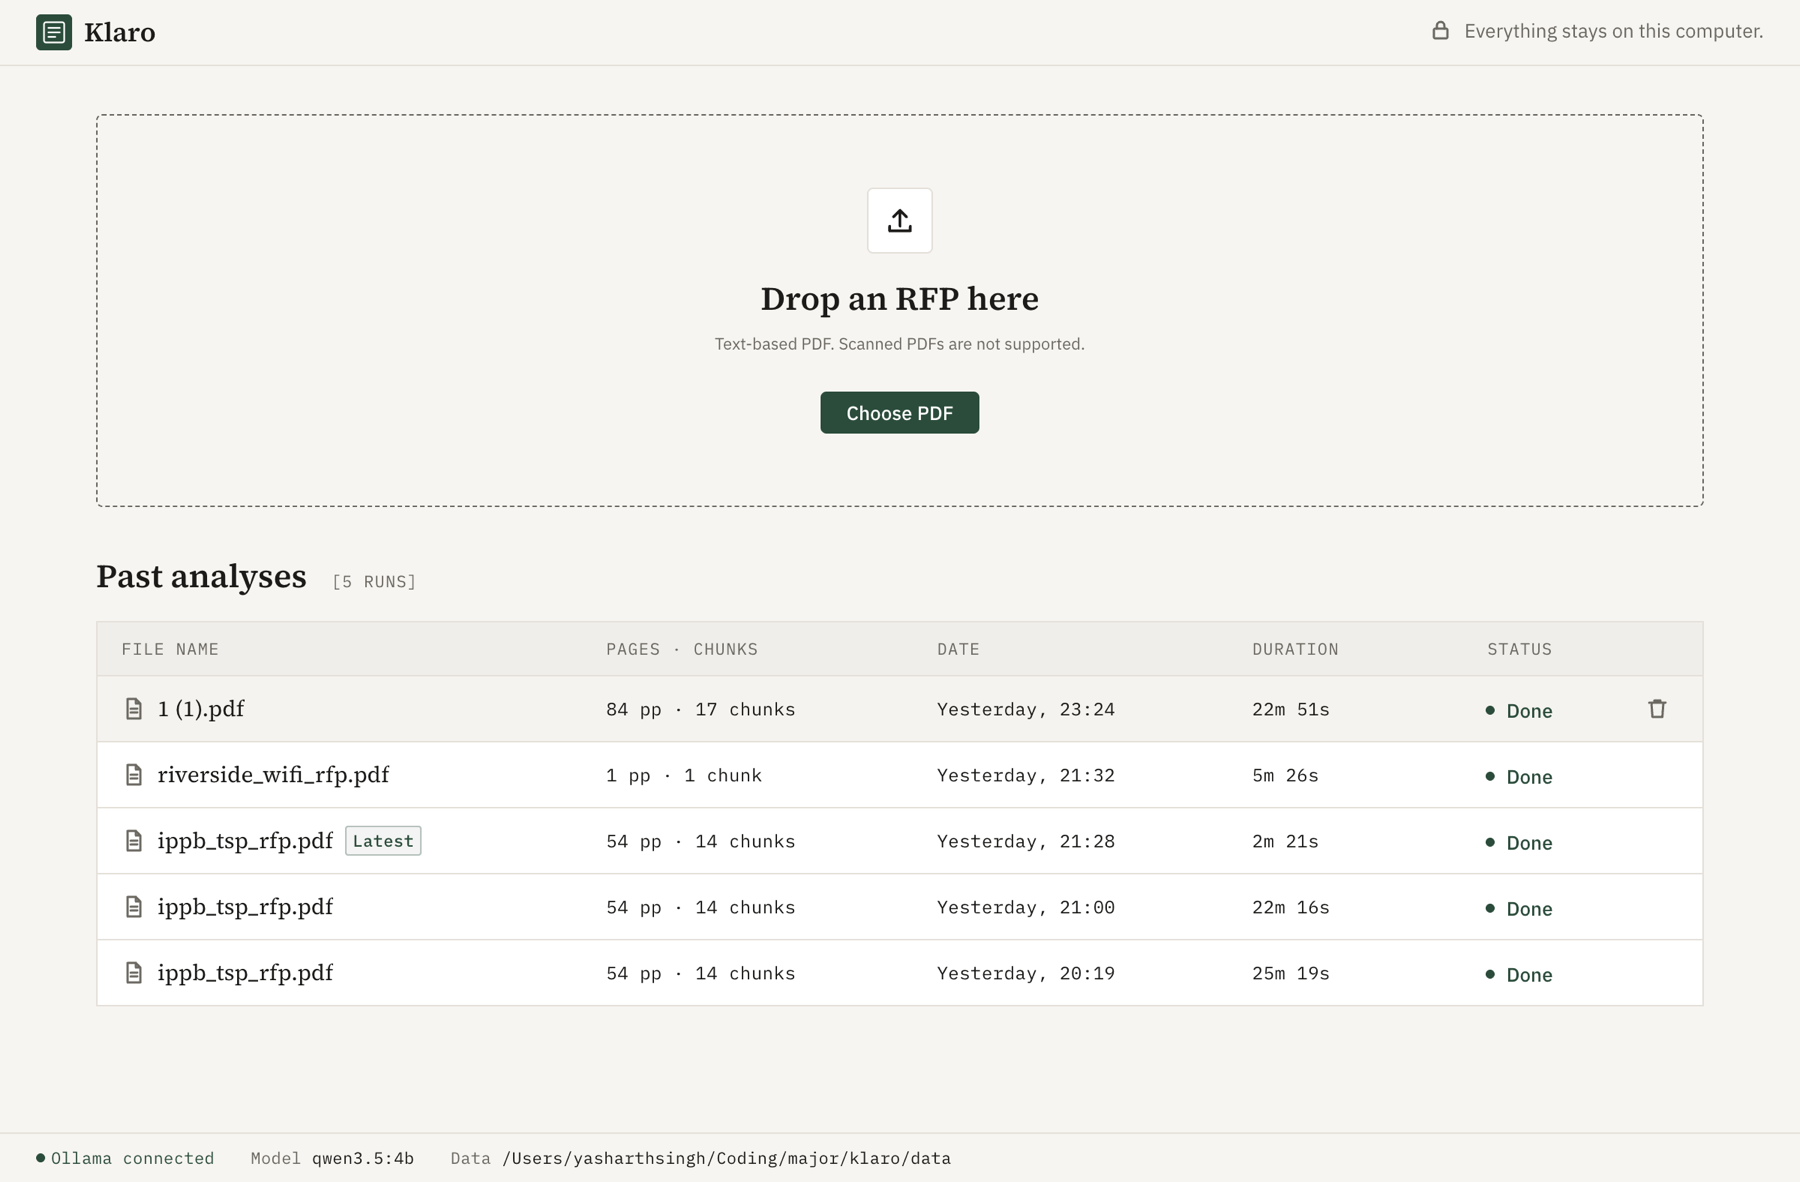
\includegraphics[width=0.86\linewidth]{figures/home.png}
\caption{Home screen: add an RFP, see past analyses and whether the AI model is ready}
\label{fig:home}
\end{figure}

\begin{figure}[H]
\centering
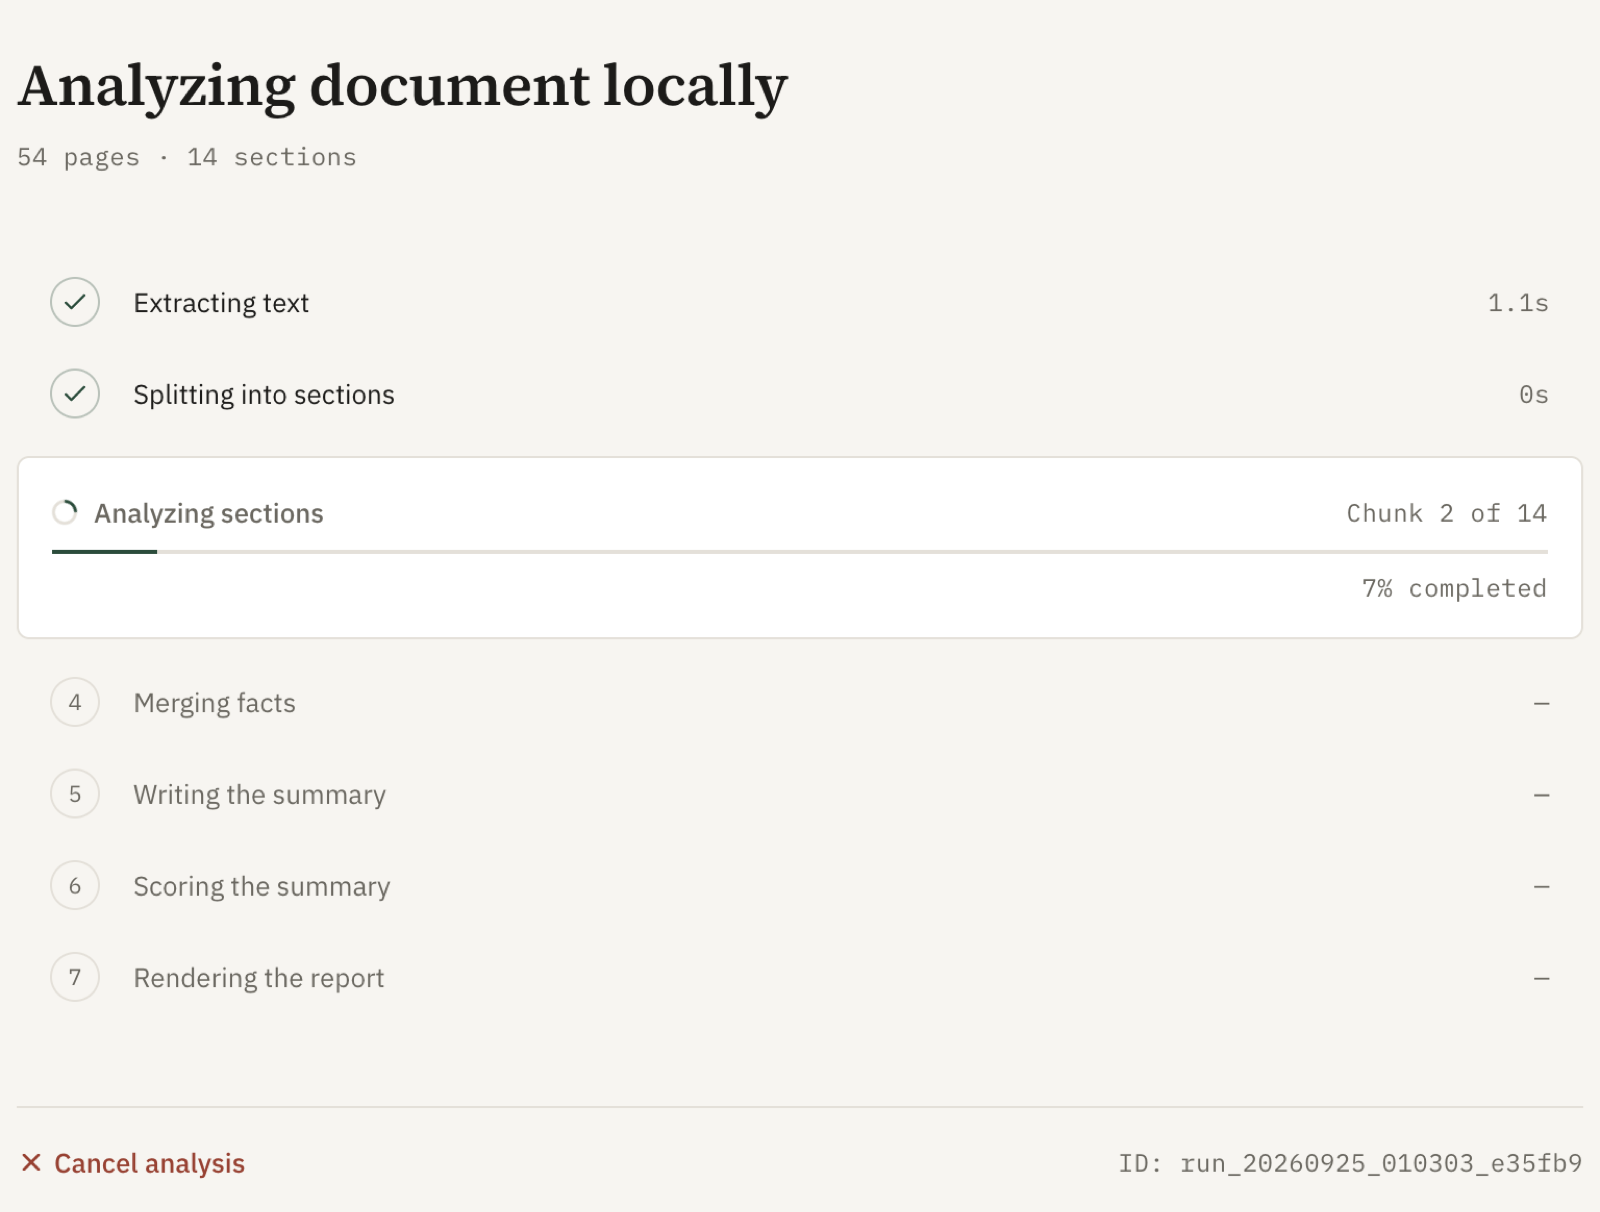
\includegraphics[width=0.66\linewidth]{figures/progress.png}
\caption{Progress screen while a 54-page RFP is being analyzed}
\label{fig:progress}
\end{figure}

\section{Testing}
Fifteen automatic tests check the report pages, the order of the pipeline steps, the handling of
failed parts, and issuer detection. All fifteen pass. The AI steps were tested end to end on the
documents in Chapter~6. The app was tested by hand on macOS; a teammate tests it on Windows.

% ------------------------------------------------------------ CHAPTER 6
\chapter{EXPERIMENTAL RESULTS AND ANALYSIS}

\section{Choosing the AI Model}
We compared three small models that can run on a laptop: Gemma~4 (e4b), Qwen3.5 (4B) and Phi-4-mini.
Each was given the same 20 RFP parts and asked to list the requirements in them. Team members had
already marked 47 requirements in those parts by hand, and each model's list was compared with this
answer sheet. A requirement counted as found (a match, at an 80\% wording-similarity threshold) when
the model's wording closely matched the hand-marked one, and standard information-retrieval metrics
were computed from that: precision, recall and F1-score. All three models used the same instructions. Tables~\ref{tab:bench-acc} to
\ref{tab:bench-fmt} break the results into accuracy, size and speed, and output format, and
Figure~\ref{fig:bench} compares the main scores.

\begin{table}[H]
\centering
\caption{Model benchmark: accuracy (47 hand-marked requirements)}
\label{tab:bench-acc}
\small
\begin{tabularx}{\linewidth}{@{}Lccc@{}}
\toprule
 & Gemma 4 (e4b) & \textbf{Qwen3.5 (4B)} & Phi-4-mini\\
\midrule
Requirements found (out of 47) & 33 & 23 & 7\\
Wrong or extra items listed & 22 & \textbf{8} & 9\\
Precision (correct when it listed something) & 60\% & \textbf{74\%} & 44\%\\
Recall (share of requirements found) & \textbf{70\%} & 49\% & 15\%\\
F1-score (balance of precision and recall) & \textbf{65\%} & 59\% & 22\%\\
Mandatory vs.\ optional judged correctly & 85\% & \textbf{91\%} & 57\%\\
Made-up requirements & 0\% & 0\% & 6\%\\
\bottomrule
\end{tabularx}
\end{table}

\begin{table}[H]
\centering
\caption{Model benchmark: size, speed and memory}
\label{tab:bench-speed}
\small
\begin{tabularx}{\linewidth}{@{}Lccc@{}}
\toprule
 & Gemma 4 (e4b) & Qwen3.5 (4B) & Phi-4-mini\\
\midrule
Model size (billions of parameters) & 8.0 & 4.7 & 3.8\\
Download size on disk (GB) & 9.6 & 3.4 & 2.5\\
Typical time per part (seconds) & 6.7 & 8.1 & 1.3\\
Slowest parts, 95th percentile (seconds) & 15.9 & 22.7 & 18.7\\
Writing speed (word pieces per second) & 28.5 & 19.0 & 48.5\\
Peak memory used (GB) & 4.4 & 6.0 & 4.3\\
\bottomrule
\end{tabularx}
\end{table}

\begin{table}[H]
\centering
\caption{Model benchmark: following the answer format}
\label{tab:bench-fmt}
\small
\begin{tabularx}{\linewidth}{@{}Lccc@{}}
\toprule
 & Gemma 4 (e4b) & Qwen3.5 (4B) & Phi-4-mini\\
\midrule
Answer usable after tolerant reading & 100\% & 100\% & 100\%\\
Answer in exactly the requested format & 45\% & 0\% & 35\%\\
Answer given as a bare list instead & 0\% & 30\% & 65\%\\
\bottomrule
\end{tabularx}
\end{table}

\begin{figure}[H]
\centering
\begin{tikzpicture}
\begin{axis}[
  ybar, bar width=9pt, width=12cm, height=5.6cm,
  ymin=0, ymax=100, ylabel={\small percent},
  symbolic x coords={G,Q,P},
  xtick=data, xticklabels={Gemma 4 (e4b), Qwen3.5 (4B), Phi-4-mini}, xticklabel style={font=\small}, yticklabel style={font=\small},
  enlarge x limits=0.25,
  legend style={font=\scriptsize, at={(0.5,1.03)}, anchor=south, legend columns=-1, draw=none},
  nodes near coords, nodes near coords style={font=\tiny},
]
\addplot[fill=cStep!60, draw=cStep] coordinates {(G,60) (Q,74) (P,44)};
\addplot[fill=cAI!60, draw=cAI] coordinates {(G,70) (Q,49) (P,15)};
\addplot[fill=cData!60, draw=cData] coordinates {(G,85) (Q,91) (P,57)};
\legend{precision, recall, mandatory/optional correct}
\end{axis}
\end{tikzpicture}
\caption{Main benchmark scores of the three models}
\label{fig:bench}
\end{figure}

\textbf{Why we chose Qwen3.5.} Phi-4-mini was fastest but found only 7 of 47 requirements and was the
only model that made one up, so it was ruled out. Between the other two, Gemma found more requirements
and was faster, which gave it the higher overall score, but it is a much bigger model: 8 billion
parameters and a 9.6 GB download, almost three times Qwen's 3.4 GB (4.7 billion parameters). Every
user has to download and store the model, so a smaller model makes Klaro practical on ordinary
laptops with limited disk space. Qwen was the more careful model: when it
listed something it was right 74\% of the time against Gemma's 60\%, it listed 8 wrong items against
Gemma's 22, and it was best at telling mandatory from optional requirements. For a summary that people
will rely on, a wrong point does more harm than a missing one, because a missing point can be found by
asking more focused questions (which is why Klaro asks two sets of questions per part), while a wrong
point may go unnoticed. Qwen's weakness in following the exact answer format is handled by Klaro's
tolerant reading of answers. Because the model is chosen in one setting, Gemma can be swapped in for a
comparison at any time; later tests with improved instructions raised Gemma's overall score to 67\%,
so it remains the main alternative.

\section{First Experiments and the Pilot Run}
Before the benchmark, the first attempt asked the model for all requirements in a part with a single
question. On five parts, two answers were empty, one was cut off and unusable, and single answers
took 2--10 minutes. This led to the two-question design. The first full run of that design on the
84-page RFP, by a teammate, gave a summary of 51 points; every point was backed by the extracted facts
and had a page number, no information was made up, 76\% of the facts were included, and the summary
was 36\% shorter than the facts. Nine points were under the wrong heading, for example a CMMI
certificate listed under conditions instead of eligibility.

\section{Full Runs through the Desktop App}
We then ran the finished app on two RFPs across three runs: an 84-page government RFP for software
development services (R1), and a 54-page bank RFP for a technical service provider, run twice
(R2, R3). Table~\ref{tab:runs} shows the results.

\begin{table}[H]
\centering
\caption{Results of the full runs (Apple M4 laptop)}
\label{tab:runs}
\small
\begin{tabularx}{\linewidth}{@{}Lccc@{}}
\toprule
 & R1 & R2 & R3\\
\midrule
Pages & 84 & 54 & 54\\
Parts analyzed & 17 & 14 & 14\\
Total time & 22 min 51 s & 25 min 19 s & 22 min 16 s\\
Points in the summary & 170 & 211 & 216\\
Points backed by facts / with page numbers & 100\% / 100\% & 100\% / 100\% & 100\% / 100\%\\
Facts included in the summary & 99\% & 97\% & 96\%\\
Shorter than the facts by & 8\% & 8\% & 9\%\\
Made-up information & none & none & none\\
Parts where the AI failed & 0 & 0 & 0\\
\bottomrule
\end{tabularx}
\end{table}

\section{What the Results Show}
\subsection{Time Taken}
About 95\% of the time goes into step 3, where the AI reads each part twice: about 1.5 minutes per part.
Writing the summary takes about one more minute. A 50--85 page RFP therefore takes 22--25 minutes,
which is why the progress screen shows which part is being read and roughly how long is left.

\subsection{Why Some Scores Look Too Good}
When we compared the files, every point under the seven list headings was an exact copy of
a collected fact: for long RFPs the model wrote only the overview, and the safety step of Section~5.5
filled in the rest. So the summary for a long RFP is currently the cleaned-up list of facts rather
than a real summary, and the ``100\% backed by facts'' score is high partly because of that copying.
The most likely reason is that the list of facts for a long RFP is too long for the amount of text the
model is set up to read at once. We have not confirmed this yet; it is the first fix planned for Phase~2.

\subsection{Same Document, Different Answers}
R2 and R3 were the same PDF, but the AI found 236 facts the first time and 244 the second, and the
number of points under some headings differed by up to ten. The model does not give identical answers on
every run, so improvements must be judged over several runs, not one.

\subsection{Issuer Detection}
With the original code, the bank RFP would have been credited to the government agency of our first
test document. After the fix, the same saved facts gave ``India Post Payments Bank Limited'', with the
ten pages where the name appears (Figure~\ref{fig:results}).

\subsection{Checking the Summary}
Every point shows its page numbers; clicking one opens the PDF at that page on the right
(Figure~\ref{fig:results}). The Quality tab shows the automatic checks with a note that they compare
words, not meaning (Figure~\ref{fig:quality}). During all runs, the app made no internet connections.

\begin{figure}[H]
\centering
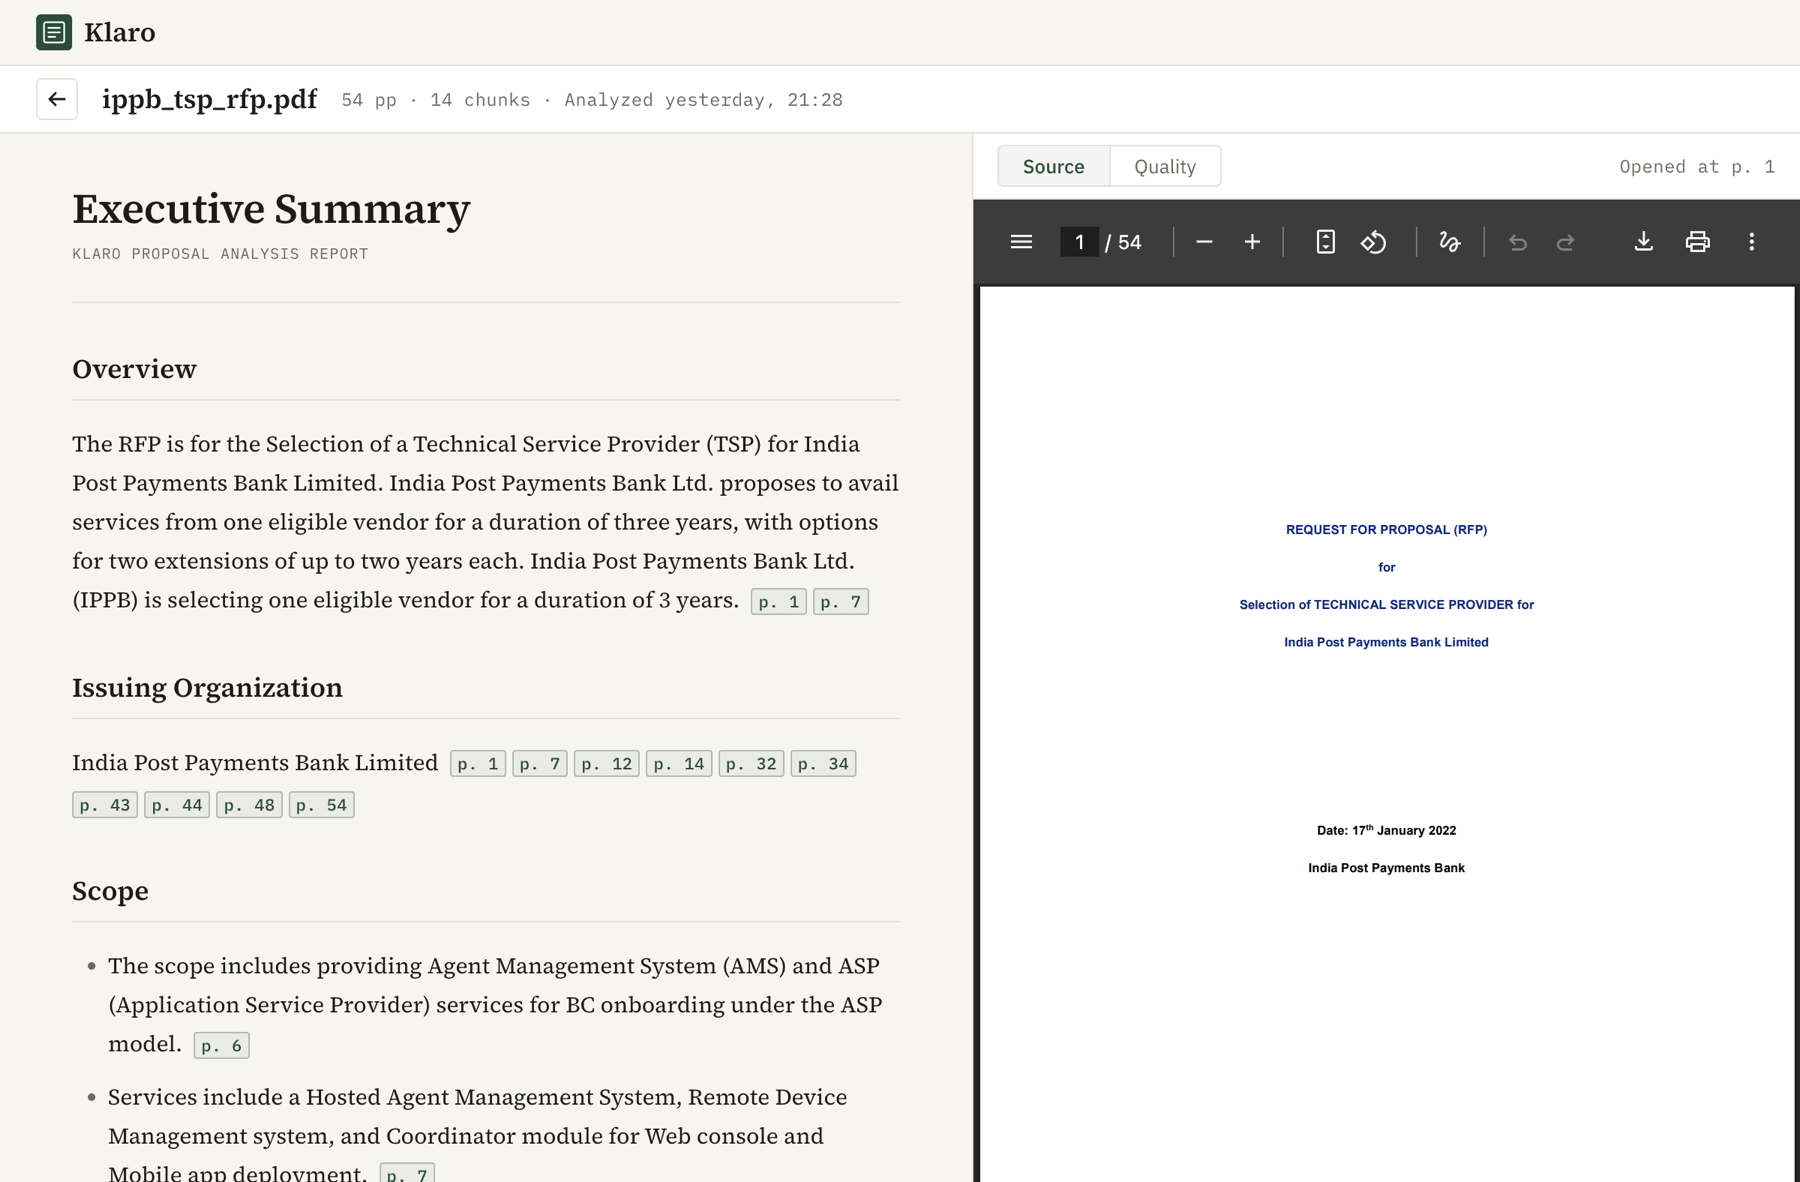
\includegraphics[width=\linewidth]{figures/results_source.png}
\caption{Results screen: summary with page numbers beside the original PDF}
\label{fig:results}
\end{figure}

\begin{figure}[H]
\centering
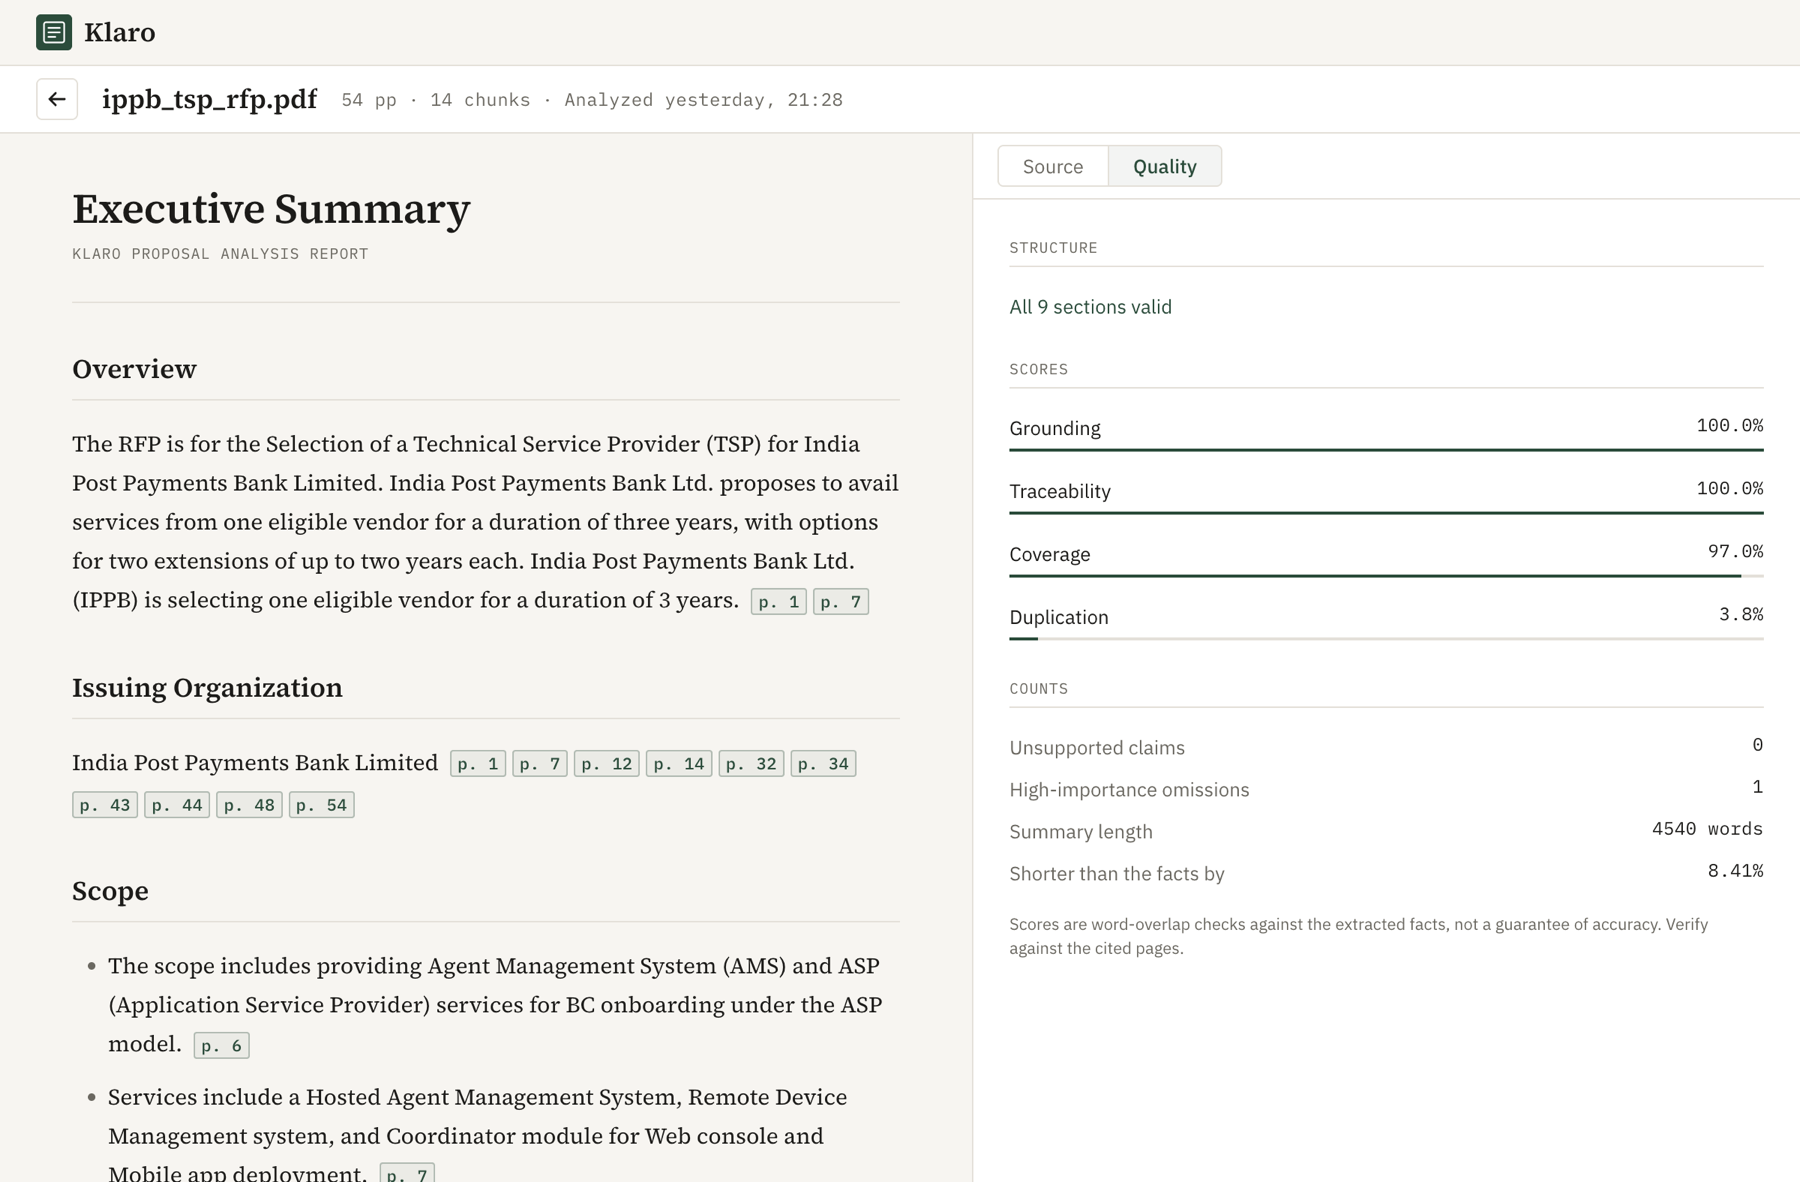
\includegraphics[width=\linewidth]{figures/results_quality.png}
\caption{Results screen with the automatic quality checks}
\label{fig:quality}
\end{figure}

% ------------------------------------------------------------ CHAPTER 7
\chapter{CONCLUSION AND FUTURE SCOPE}

\section{Conclusion}
Klaro's first phase works end to end: a 54--84 page tender goes in, and 22--25 minutes later a
nine-heading summary comes out on an ordinary laptop, with a page number on every point and nothing
sent over the internet. We chose the AI model by testing three on the same task, and chose Qwen3.5
because it made the fewest wrong claims and is about a third of the size of the closest competitor. The same process runs from the command line for testing and
inside a desktop app for analysts, and when something goes wrong (the model is missing, the PDF is a
scan, the AI fails on too many parts) the app says so clearly. Testing also showed where the system
falls short, mainly that summaries of long RFPs are not yet shortened, and those findings set the
order of work for the next phase.

\section{Limitations}
\begin{itemize}
\item Only three RFPs were tested, so we cannot yet say how well it works on tenders in general.
\item There are no human-written reference summaries yet to compare against.
\item Summaries of long RFPs are not yet shortened (Section~6.4.2).
\item The AI can give different answers on different runs, and 22--25 minutes is slow.
\item Only English, text-based PDFs work; tables lose their layout.
\item There is no installer yet; the app runs from the project folder.
\end{itemize}

\section{Future Scope}
\subsection{Proposal Assistant}
Klaro will grow into a Proposal Assistant with two ways of working (Figure~\ref{fig:future}). In the
\textbf{agentic workflow}, three AI helpers share the same reading of the RFP: the existing Executive
Summary agent, a Requirements agent that produces a checklist of what the bidder must do, and a
Starter Pack agent that turns the analysis into a first outline of the proposal, with risks and
questions to ask the client. In the \textbf{file search workflow}, the company's past proposals and case
studies are indexed on the laptop, and the ones most similar to a new RFP are found and handed to the
Starter Pack agent.

\begin{figure}[H]
\centering
\begin{tikzpicture}
\node[term, text width=2.2cm] (rfp) at (0,0) {New RFP};
\node[data, text width=3.2cm] (ctx) at (3.9,0) {\st{Shared reading}{parts and extracted facts}};
\node[ai, text width=4.1cm] (ag1) at (8.6,1.35) {Requirements agent};
\node[ai, text width=4.1cm] (ag2) at (8.6,0) {Executive Summary agent};
\node[ai, text width=4.1cm] (ag3) at (8.6,-1.35) {Starter Pack agent};
\node[zone, fit=(ag1)(ag2)(ag3), label={[ztitle]above:1. Agentic workflow}] (g1) {};
\node[user, text width=2.4cm] (out) at (13.3,0) {\st{Results}{checklist, summary, proposal draft}};
\node[data, text width=3.2cm] (lib) at (3.9,-3.4) {\st{Past proposals}{and case studies}};
\node[proc, text width=3.3cm] (srch) at (8.6,-3.4) {\st{Search}{find the most similar ones}};
\node[zone, fit=(lib)(srch), label={[ztitle]below:2. File search workflow}] (g2) {};
\draw[arr] (rfp) -- (ctx);
\foreach \a in {ag1,ag2,ag3} { \draw[arr] (ctx.east) -- (\a.west); \draw[arr] (\a.east) -- (out.west); }
\draw[arr] (lib) -- (srch);
\draw[arr] (ctx) -- node[lbl, left]{what to look for} (lib);
\draw[arr] (srch) -- node[lbl, right]{relevant examples} (g1.south -| srch);
\end{tikzpicture}
\caption{The planned Proposal Assistant}
\label{fig:future}
\end{figure}

\subsection{Real-Time Progress Updates}
Today the app shows which step and which part it is working on. The next step is to show the results
of each step as they are produced, so users do not wait for the final result: facts appear under
their headings as each part is read, the summary appears as the model writes it, and the Starter Pack
fills in section by section.

\subsection{Better Summaries and Better Testing}
\begin{itemize}
\item Fix the long-document problem: let the model read more at once, write one heading at a time,
      and record when the safety copy is used.
\item Collect 30--40 real RFPs and build a reference set: a larger LLM drafts a first summary for
      each one, a human then corrects it, and the corrected version becomes the golden summary used
      to test every future change.
\item Fine-tune Qwen3.5 with LoRA, a low-cost way to further train a model without retraining it in
      full, on these golden summaries, instead of
      relying only on prompting, and compare the fine-tuned model with the current one on the same
      benchmark. This targets the copying problem of Section~6.4.2: a model that has actually seen
      the summarization task, not just an instruction describing it, should need less safety-copy
      fallback and produce a genuinely shorter summary on long RFPs.
\item Repeat the model benchmark on the summary task, with Gemma~4 as the main alternative.
\end{itemize}

\subsection{App Improvements}
\begin{itemize}
\item One-click installers for Windows and macOS, with guided setup of the AI model.
\item Support for Word files, scanned PDFs and tables.
\item Multilingual support, starting with German: read German RFPs and write the summary in German or English, since the multilingual extension was planned from the start.
\item Let users accept, edit or flag each point, and use that feedback to measure quality.
\end{itemize}

% ------------------------------------------------------------ REFERENCES
\cleardoublepage
\addtocontents{toc}{\protect\vspace{6pt}}
\addtocline{\bfseries}{References}
\renewcommand{\bibname}{REFERENCES}
\begin{singlespace}
\small
\bibliographystyle{IEEEtran}
\bibliography{references}
\end{singlespace}

\end{document}
